\documentclass[10pt,a4paper]{article}
\usepackage[utf8]{inputenc}
\usepackage[russian]{babel}
\usepackage[OT1]{fontenc}
\usepackage{amsmath}
\usepackage{amsfonts}
\usepackage{amssymb}
\usepackage{graphicx}
\graphicspath{{Images/}}
\usepackage[left=2cm,right=2cm,top=2cm,bottom=2cm]{geometry}
\usepackage{calc}
\usepackage{wrapfig}
\usepackage{setspace}
\usepackage{indentfirst}
\usepackage{subfigure}
\usepackage{multirow}
\usepackage{longtable}


\title{
Отчет о выполнении лабораторной работы 3.2.5

Вынужденные колебания в электрическом контуре
}

\author{Варламов Антоний, группа Б02-928}

\begin{document}

\maketitle

\newpage

	\section{Введение}
	
	\textit{Цель работы:} Исследование вынужденных колебаний в электрическом контуре и процессов их установления.
	
	\textit{Оборудование:} генератор звуковой частоты, осциллограф, вольтметр, частотометр, конденсатор, катушка индуктивности, магазин сопротивлений.
	
	\begin{wrapfigure}[9]{r}{0.23\textwidth}
		\vspace{-0.5cm}
		\centering
		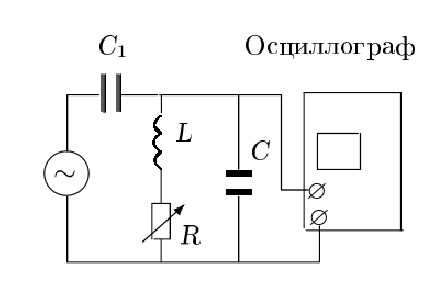
\includegraphics[width = 0.2\textwidth]{schem_of_circuit}
		\caption{Схема исследуемого контура}
		\label{fig:schem_of_circuit}
	\end{wrapfigure}
	
	В работе исследуются вынужденные колебания, возникающие в электрическом контуре (рис \ref{fig:schem_of_circuit}) при подаче на него переменного ЭДС, гармонически изменяющегося со временем. При этом, параметры колебаний будут зависеть как от параметров самого контура -- индуктивности катушки, емкости конденсатора, а также его сопротивления, так и от параметров источника ЭДС -- частоты колебания ЭДС и амплитуды данных колебаний. Основное явление, которое можно наглядным образом наблюдать в подобной системе -- явление резонанса. Резонанс -- явление резкого увеличения амплитуды вынужденных колебаний при частотах источника ЭДС близких к собственной частоте контура.
	
	Кривая, описывающая зависимость амплитуды вынужденных колебаний от частоты источника ЭДС называется резонансной кривой. Первая часть работы будет посвящена исследованию резонансных кривых для контура в двух конфигурациях -- при наличии постоянного сопротивления контура и при его отсутствии.
	
	Исследование резонансных кривых позволит определить \textit{добротность} контура в различных конфигурациях. 
	
	Для этого можно воспользоваться формулой:
	
	\begin{equation}
		Q = \frac{\omega_{0}}{2\Delta \Omega}
		\label{eq:equation_1}
	\end{equation}
	
	где $\omega_{0}$ -- собственная частота контура, $\Delta \Omega = \left|\Omega - \omega_{0} \right|$. 
	
	\begin{wrapfigure}[8]{r}{0.23\textwidth}
		\vspace{-1.5cm}
		\centering
		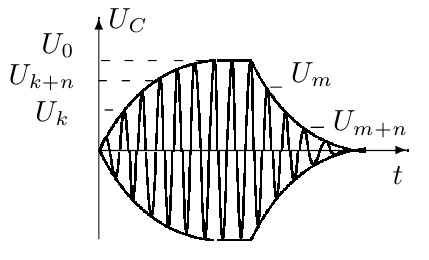
\includegraphics[width = 0.2\textwidth]{graph_of_depence_amplitude}
		\caption{График зависимости амплитуды от времени}
		\label{fig:graph_of_depence_amplitude}
	\end{wrapfigure}\vspace{0.5cm}
	
	Другим же методом, который позволит определить добротность контура является метод исследования процессов установления и затухания колебаний. Данный метод основан на исследовании зависимости амплитуды колебаний в процессе затухания или установления колебаний. График зависимости амплитуды от времени приведен на (рис. \ref{fig:graph_of_depence_amplitude}). В этом случае очень удобно можно получить логарифмический декремент затухания:
	
	\begin{equation}
		\Theta = \frac{1}{n}\ln \left(\frac{U_{0} - U_{k}}{U_{0} - U_{k + n}}\right)
		\label{eq:equation_2}
	\end{equation}
	
	Зная логарифмический декремент затухания, нетрудно выразить добротность контура:
	
	\begin{equation}
		Q = \frac{\pi}{\Theta}
		\label{eq:equation_3}
	\end{equation}
	
	\section{Схема установки}
	\begin{figure}[h!]	
		\begin{center}
			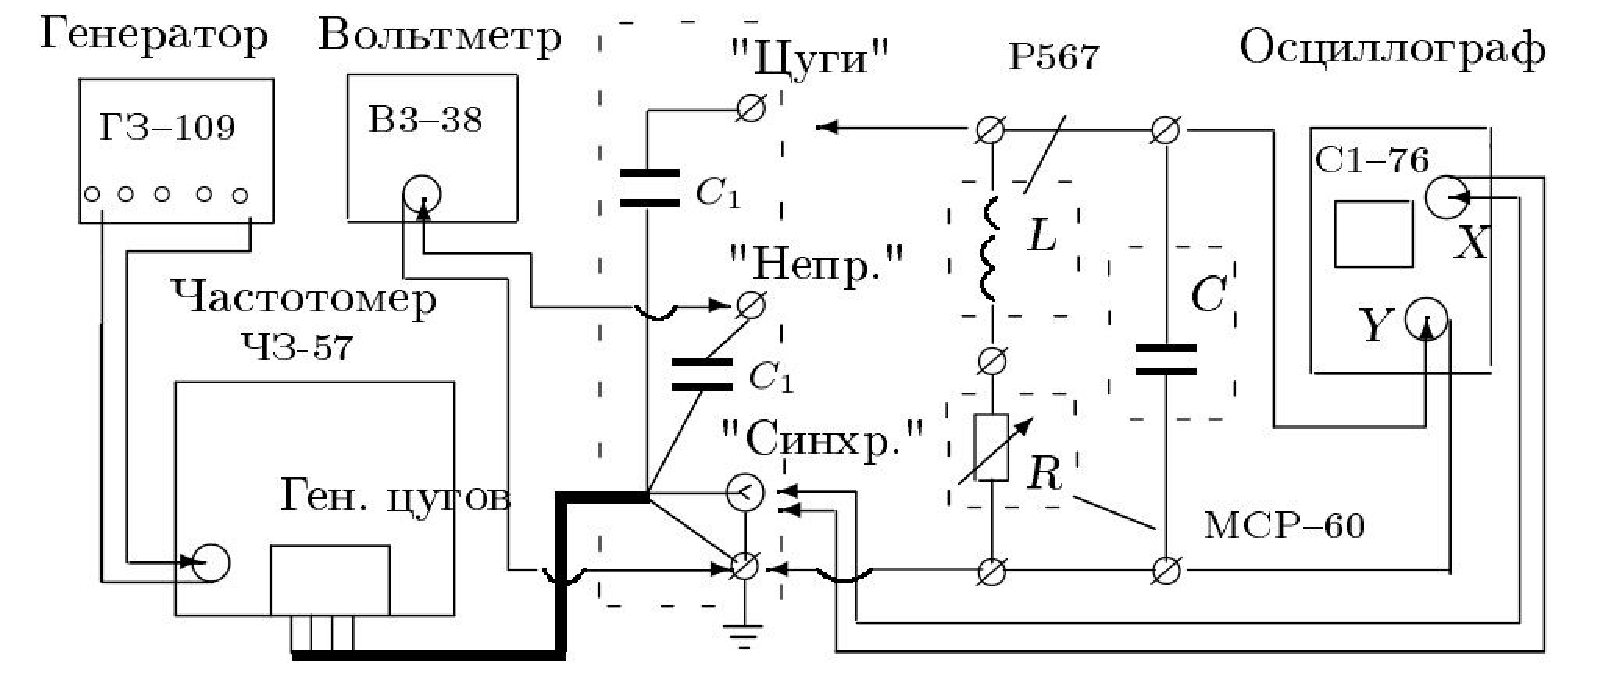
\includegraphics[width = 0.75\textwidth]{schem_of_facility}
			\caption{Схема установки}
			\label{fig:schem_of_facility}
		\end{center}
	\end{figure}
	
	\section{Ход выполнения работы}
	\subsection{Построение резонансных кривых}
	
	\begin{table}[h!]
\centering
\begin{tabular}{|l|l|l|l|llllllll}
\hline
\multicolumn{6}{|c|}{$R = 0$ Ом} &
  \multicolumn{6}{c|}{$R = 100$ Ом} \\ \hline
$\nu$, Гц &
  $U$,  В &
  $\nu$, Гц &
  $U$,  В &
  \multicolumn{1}{l|}{$\nu$, Гц} &
  \multicolumn{1}{l|}{$U$,  В} &
  \multicolumn{1}{l|}{$\nu$, Гц} &
  \multicolumn{1}{l|}{$U$,  мВ} &
  \multicolumn{1}{l|}{$\nu$, Гц} &
  \multicolumn{1}{l|}{$U$,  мВ} &
  \multicolumn{1}{l|}{$\nu$, Гц} &
  \multicolumn{1}{l|}{$U$,  мВ} \\ \hline
1569 &
  30,0 &
  1629 &
  30,0 &
  \multicolumn{1}{l|}{1621} &
  \multicolumn{1}{l|}{23,0} &
  \multicolumn{1}{l|}{1600} &
  \multicolumn{1}{l|}{300} &
  \multicolumn{1}{l|}{1598} &
  \multicolumn{1}{l|}{300} &
  \multicolumn{1}{l|}{1466} &
  \multicolumn{1}{l|}{174} \\ \hline
1563 &
  29,5 &
  1630 &
  29,5 &
  \multicolumn{1}{l|}{1623} &
  \multicolumn{1}{l|}{22,5} &
  \multicolumn{1}{l|}{1627} &
  \multicolumn{1}{l|}{294} &
  \multicolumn{1}{l|}{1580} &
  \multicolumn{1}{l|}{294} &
  \multicolumn{1}{l|}{1472} &
  \multicolumn{1}{l|}{180} \\ \hline
1562 &
  29,0 &
  1631 &
  29,0 &
  \multicolumn{1}{l|}{1624} &
  \multicolumn{1}{l|}{22,0} &
  \multicolumn{1}{l|}{1637} &
  \multicolumn{1}{l|}{288} &
  \multicolumn{1}{l|}{1569} &
  \multicolumn{1}{l|}{288} &
  \multicolumn{1}{l|}{1479} &
  \multicolumn{1}{l|}{186} \\ \hline
1562 &
  28,5 &
  1632 &
  28,5 &
  \multicolumn{1}{l|}{1625} &
  \multicolumn{1}{l|}{21,5} &
  \multicolumn{1}{l|}{1645} &
  \multicolumn{1}{l|}{282} &
  \multicolumn{1}{l|}{1562} &
  \multicolumn{1}{l|}{282} &
  \multicolumn{1}{l|}{1484} &
  \multicolumn{1}{l|}{192} \\ \hline
1560 &
  28,0 &
  1633 &
  28,0 &
  \multicolumn{1}{l|}{1626} &
  \multicolumn{1}{l|}{21,0} &
  \multicolumn{1}{l|}{1652} &
  \multicolumn{1}{l|}{276} &
  \multicolumn{1}{l|}{1555} &
  \multicolumn{1}{l|}{276} &
  \multicolumn{1}{l|}{1490} &
  \multicolumn{1}{l|}{198} \\ \hline
1559 &
  27,5 &
  1635 &
  27,5 &
  \multicolumn{1}{l|}{1628} &
  \multicolumn{1}{l|}{20,5} &
  \multicolumn{1}{l|}{1659} &
  \multicolumn{1}{l|}{270} &
  \multicolumn{1}{l|}{1550} &
  \multicolumn{1}{l|}{270} &
  \multicolumn{1}{l|}{1495} &
  \multicolumn{1}{l|}{204} \\ \hline
1558 &
  27,0 &
  1635 &
  27,0 &
  \multicolumn{1}{l|}{1630} &
  \multicolumn{1}{l|}{20,0} &
  \multicolumn{1}{l|}{1665} &
  \multicolumn{1}{l|}{264} &
  \multicolumn{1}{l|}{1545} &
  \multicolumn{1}{l|}{264} &
  \multicolumn{1}{l|}{1502} &
  \multicolumn{1}{l|}{210} \\ \hline
1557 &
  26,5 &
  1636 &
  26,5 &
  \multicolumn{1}{l|}{1633} &
  \multicolumn{1}{l|}{19,5} &
  \multicolumn{1}{l|}{1673} &
  \multicolumn{1}{l|}{258} &
  \multicolumn{1}{l|}{1540} &
  \multicolumn{1}{l|}{258} &
  \multicolumn{1}{l|}{1505} &
  \multicolumn{1}{l|}{216} \\ \hline
1556 &
  26,0 &
  1638 &
  26,0 &
  \multicolumn{1}{l|}{1634} &
  \multicolumn{1}{l|}{19,0} &
  \multicolumn{1}{l|}{1679} &
  \multicolumn{1}{l|}{252} &
  \multicolumn{1}{l|}{1534} &
  \multicolumn{1}{l|}{252} &
  \multicolumn{1}{l|}{1509} &
  \multicolumn{1}{l|}{222} \\ \hline
1555 &
  25,5 &
  1639 &
  25,5 &
  \multicolumn{1}{l|}{1637} &
  \multicolumn{1}{l|}{18,5} &
  \multicolumn{1}{l|}{1686} &
  \multicolumn{1}{l|}{246} &
  \multicolumn{1}{l|}{1531} &
  \multicolumn{1}{l|}{246} &
  \multicolumn{1}{l|}{1515} &
  \multicolumn{1}{l|}{228} \\ \hline
1554 &
  25,0 &
  1640 &
  25,0 &
  \multicolumn{1}{l|}{1638} &
  \multicolumn{1}{l|}{18,0} &
  \multicolumn{1}{l|}{1692} &
  \multicolumn{1}{l|}{240} &
  \multicolumn{1}{l|}{1526} &
  \multicolumn{1}{l|}{240} &
  \multicolumn{1}{l|}{1520} &
  \multicolumn{1}{l|}{234} \\ \hline
1553 &
  24,5 &
  1642 &
  24,5 &
  \multicolumn{1}{l|}{1638} &
  \multicolumn{1}{l|}{17,5} &
  \multicolumn{1}{l|}{1700} &
  \multicolumn{1}{l|}{234} &
  \multicolumn{1}{l|}{1519} &
  \multicolumn{1}{l|}{234} &
  \multicolumn{1}{l|}{1524} &
  \multicolumn{1}{l|}{240} \\ \hline
1551 &
  24,0 &
  1643 &
  24,0 &
  \multicolumn{1}{l|}{1640} &
  \multicolumn{1}{l|}{17,0} &
  \multicolumn{1}{l|}{1707} &
  \multicolumn{1}{l|}{228} &
  \multicolumn{1}{l|}{1515} &
  \multicolumn{1}{l|}{228} &
  \multicolumn{1}{l|}{1530} &
  \multicolumn{1}{l|}{246} \\ \hline
1550 &
  23,5 &
  1645 &
  23,5 &
  \multicolumn{1}{l|}{1556} &
  \multicolumn{1}{l|}{17,5} &
  \multicolumn{1}{l|}{1714} &
  \multicolumn{1}{l|}{222} &
  \multicolumn{1}{l|}{1510} &
  \multicolumn{1}{l|}{222} &
  \multicolumn{1}{l|}{1686} &
  \multicolumn{1}{l|}{246} \\ \hline
1549 &
  23,0 &
  1646 &
  23,0 &
  \multicolumn{1}{l|}{1558} &
  \multicolumn{1}{l|}{18,0} &
  \multicolumn{1}{l|}{1719} &
  \multicolumn{1}{l|}{216} &
  \multicolumn{1}{l|}{1503} &
  \multicolumn{1}{l|}{216} &
  \multicolumn{1}{l|}{1692} &
  \multicolumn{1}{l|}{240} \\ \hline
1548 &
  22,5 &
  1648 &
  22,5 &
  \multicolumn{1}{l|}{1559} &
  \multicolumn{1}{l|}{18,5} &
  \multicolumn{1}{l|}{1728} &
  \multicolumn{1}{l|}{210} &
  \multicolumn{1}{l|}{1500} &
  \multicolumn{1}{l|}{210} &
  \multicolumn{1}{l|}{1699} &
  \multicolumn{1}{l|}{234} \\ \hline
1546 &
  22,0 &
  1649 &
  22,0 &
  \multicolumn{1}{l|}{1561} &
  \multicolumn{1}{l|}{19,0} &
  \multicolumn{1}{l|}{1737} &
  \multicolumn{1}{l|}{204} &
  \multicolumn{1}{l|}{1497} &
  \multicolumn{1}{l|}{204} &
  \multicolumn{1}{l|}{1707} &
  \multicolumn{1}{l|}{228} \\ \hline
1545 &
  21,5 &
  1651 &
  21,5 &
  \multicolumn{1}{l|}{1562} &
  \multicolumn{1}{l|}{19,5} &
  \multicolumn{1}{l|}{1744} &
  \multicolumn{1}{l|}{198} &
  \multicolumn{1}{l|}{1489} &
  \multicolumn{1}{l|}{198} &
  \multicolumn{1}{l|}{1715} &
  \multicolumn{1}{l|}{222} \\ \hline
1543 &
  21,0 &
  1653 &
  21,0 &
  \multicolumn{1}{l|}{1563} &
  \multicolumn{1}{l|}{20,0} &
  \multicolumn{1}{l|}{1754} &
  \multicolumn{1}{l|}{192} &
  \multicolumn{1}{l|}{1484} &
  \multicolumn{1}{l|}{192} &
  \multicolumn{1}{l|}{1722} &
  \multicolumn{1}{l|}{216} \\ \hline
1542 &
  20,5 &
  1654 &
  20,5 &
  \multicolumn{1}{l|}{1565} &
  \multicolumn{1}{l|}{20,5} &
  \multicolumn{1}{l|}{1763} &
  \multicolumn{1}{l|}{186} &
  \multicolumn{1}{l|}{1479} &
  \multicolumn{1}{l|}{186} &
  \multicolumn{1}{l|}{1728} &
  \multicolumn{1}{l|}{210} \\ \hline
1540 &
  20,0 &
  1656 &
  20,0 &
  \multicolumn{1}{l|}{1566} &
  \multicolumn{1}{l|}{21,0} &
  \multicolumn{1}{l|}{1773} &
  \multicolumn{1}{l|}{180} &
  \multicolumn{1}{l|}{1473} &
  \multicolumn{1}{l|}{180} &
  \multicolumn{1}{l|}{1737} &
  \multicolumn{1}{l|}{204} \\ \hline
1538 &
  19,5 &
  1658 &
  19,5 &
  \multicolumn{1}{l|}{1568} &
  \multicolumn{1}{l|}{21,5} &
  \multicolumn{1}{l|}{1784} &
  \multicolumn{1}{l|}{174} &
  \multicolumn{1}{l|}{1467} &
  \multicolumn{1}{l|}{174} &
  \multicolumn{1}{l|}{1746} &
  \multicolumn{1}{l|}{198} \\ \hline
1537 &
  19,0 &
  1661 &
  19,0 &
  \multicolumn{1}{l|}{1569} &
  \multicolumn{1}{l|}{22,0} &
  \multicolumn{1}{l|}{1795} &
  \multicolumn{1}{l|}{168} &
  \multicolumn{1}{l|}{1459} &
  \multicolumn{1}{l|}{168} &
  \multicolumn{1}{l|}{1754} &
  \multicolumn{1}{l|}{192} \\ \hline
1535 &
  18,5 &
  1663 &
  18,5 &
  \multicolumn{1}{l|}{1569} &
  \multicolumn{1}{l|}{22,5} &
  \multicolumn{1}{l|}{1807} &
  \multicolumn{1}{l|}{162} &
  \multicolumn{1}{l|}{1455} &
  \multicolumn{1}{l|}{162} &
  \multicolumn{1}{l|}{1763} &
  \multicolumn{1}{l|}{186} \\ \hline
1534 &
  18,0 &
  1665 &
  18,0 &
  \multicolumn{1}{l|}{1571} &
  \multicolumn{1}{l|}{23,0} &
  \multicolumn{1}{l|}{1819} &
  \multicolumn{1}{l|}{156} &
  \multicolumn{1}{l|}{1447} &
  \multicolumn{1}{l|}{156} &
  \multicolumn{1}{l|}{1774} &
  \multicolumn{1}{l|}{180} \\ \hline
1532 &
  17,5 &
  1668 &
  17,5 &
   &
  \multicolumn{1}{l|}{} &
  \multicolumn{1}{l|}{1833} &
  \multicolumn{1}{l|}{150} &
  \multicolumn{1}{l|}{1440} &
  \multicolumn{1}{l|}{150} &
  \multicolumn{1}{l|}{1785} &
  \multicolumn{1}{l|}{174} \\ \cline{1-4} \cline{7-12} 
1529 &
  17,0 &
  1670 &
  17,0 &
   &
  \multicolumn{1}{l|}{} &
  \multicolumn{1}{l|}{1848} &
  \multicolumn{1}{l|}{144} &
  \multicolumn{1}{l|}{1432} &
  \multicolumn{1}{l|}{144} &
   &
   \\ \cline{1-4} \cline{7-10}
1528 &
  16,5 &
  1673 &
  16,5 &
   &
  \multicolumn{1}{l|}{} &
  \multicolumn{1}{l|}{1856} &
  \multicolumn{1}{l|}{138} &
  \multicolumn{1}{l|}{1425} &
  \multicolumn{1}{l|}{138} &
   &
   \\ \cline{1-4} \cline{7-10}
1525 &
  16,0 &
  1677 &
  16,0 &
   &
  \multicolumn{1}{l|}{} &
  \multicolumn{1}{l|}{1887} &
  \multicolumn{1}{l|}{132} &
  \multicolumn{1}{l|}{1416} &
  \multicolumn{1}{l|}{132} &
   &
   \\ \cline{1-4} \cline{7-10}
1523 &
  15,5 &
  1679 &
  15,5 &
   &
  \multicolumn{1}{l|}{} &
  \multicolumn{1}{l|}{1907} &
  \multicolumn{1}{l|}{126} &
  \multicolumn{1}{l|}{1407} &
  \multicolumn{1}{l|}{126} &
   &
   \\ \cline{1-4} \cline{7-10}
1520 &
  15,0 &
  1683 &
  15,0 &
   &
  \multicolumn{1}{l|}{} &
  \multicolumn{1}{l|}{1931} &
  \multicolumn{1}{l|}{120} &
  \multicolumn{1}{l|}{1397} &
  \multicolumn{1}{l|}{120} &
   &
   \\ \cline{1-4} \cline{7-10}
1517 &
  14,5 &
  1687 &
  14,5 &
   &
  \multicolumn{1}{l|}{} &
  \multicolumn{1}{l|}{1958} &
  \multicolumn{1}{l|}{114} &
  \multicolumn{1}{l|}{1388} &
  \multicolumn{1}{l|}{114} &
   &
   \\ \cline{1-4} \cline{7-10}
1514 &
  14,0 &
  1691 &
  14,0 &
   &
  \multicolumn{1}{l|}{} &
  \multicolumn{1}{l|}{1990} &
  \multicolumn{1}{l|}{108} &
  \multicolumn{1}{l|}{1376} &
  \multicolumn{1}{l|}{108} &
   &
   \\ \cline{1-4} \cline{7-10}
1511 &
  13,5 &
  1695 &
  13,5 &
   &
  \multicolumn{1}{l|}{} &
  \multicolumn{1}{l|}{2029} &
  \multicolumn{1}{l|}{102} &
  \multicolumn{1}{l|}{1364} &
  \multicolumn{1}{l|}{102} &
   &
   \\ \cline{1-4} \cline{7-10}
1508 &
  13,0 &
  1699 &
  13,0 &
   &
  \multicolumn{1}{l|}{} &
  \multicolumn{1}{l|}{2070} &
  \multicolumn{1}{l|}{96} &
  \multicolumn{1}{l|}{1352} &
  \multicolumn{1}{l|}{96} &
   &
   \\ \cline{1-4} \cline{7-10}
1505 &
  12,5 &
  1703 &
  12,5 &
   &
   &
   &
   &
   &
   &
   &
   \\ \cline{1-4}
1502 &
  12,0 &
  1708 &
  12,0 &
   &
   &
   &
   &
   &
   &
   &
   \\ \cline{1-4}
1497 &
  11,5 &
  1716 &
  11,5 &
   &
   &
   &
   &
   &
   &
   &
   \\ \cline{1-4}
1493 &
  11,0 &
  1723 &
  11,0 &
   &
   &
   &
   &
   &
   &
   &
   \\ \cline{1-4}
1488 &
  10,5 &
  1730 &
  10,5 &
   &
   &
   &
   &
   &
   &
   &
   \\ \cline{1-4}
1484 &
  10,0 &
  1737 &
  10,0 &
   &
   &
   &
   &
   &
   &
   &
   \\ \cline{1-4}
1477 &
  9,5 &
  1746 &
  9,5 &
   &
   &
   &
   &
   &
   &
   &
   \\ \cline{1-4}
1471 &
  9,0 &
  1756 &
  9,0 &
   &
   &
   &
   &
   &
   &
   &
   \\ \cline{1-4}
1465 &
  8,5 &
  1766 &
  8,5 &
   &
   &
   &
   &
   &
   &
   &
   \\ \cline{1-4}
1458 &
  8,0 &
  1780 &
  8,0 &
   &
   &
   &
   &
   &
   &
   &
   \\ \cline{1-4}
1449 &
  7,5 &
  1795 &
  7,5 &
   &
   &
   &
   &
   &
   &
   &
   \\ \cline{1-4}
1441 &
  7,0 &
  1815 &
  7,0 &
   &
   &
   &
   &
   &
   &
   &
   \\ \cline{1-4}
\end{tabular}
\caption{Результаты измерения зависимости амплитуды напряжения колебаний в контуре при $R = 0$ Ом и $R = 100$ Ом}
\label{tab:amplitude_measuring}
\end{table}

	\begin{figure}[h!]
		\begin{minipage}{0.49\textwidth}
			\hspace{-0.5cm}
			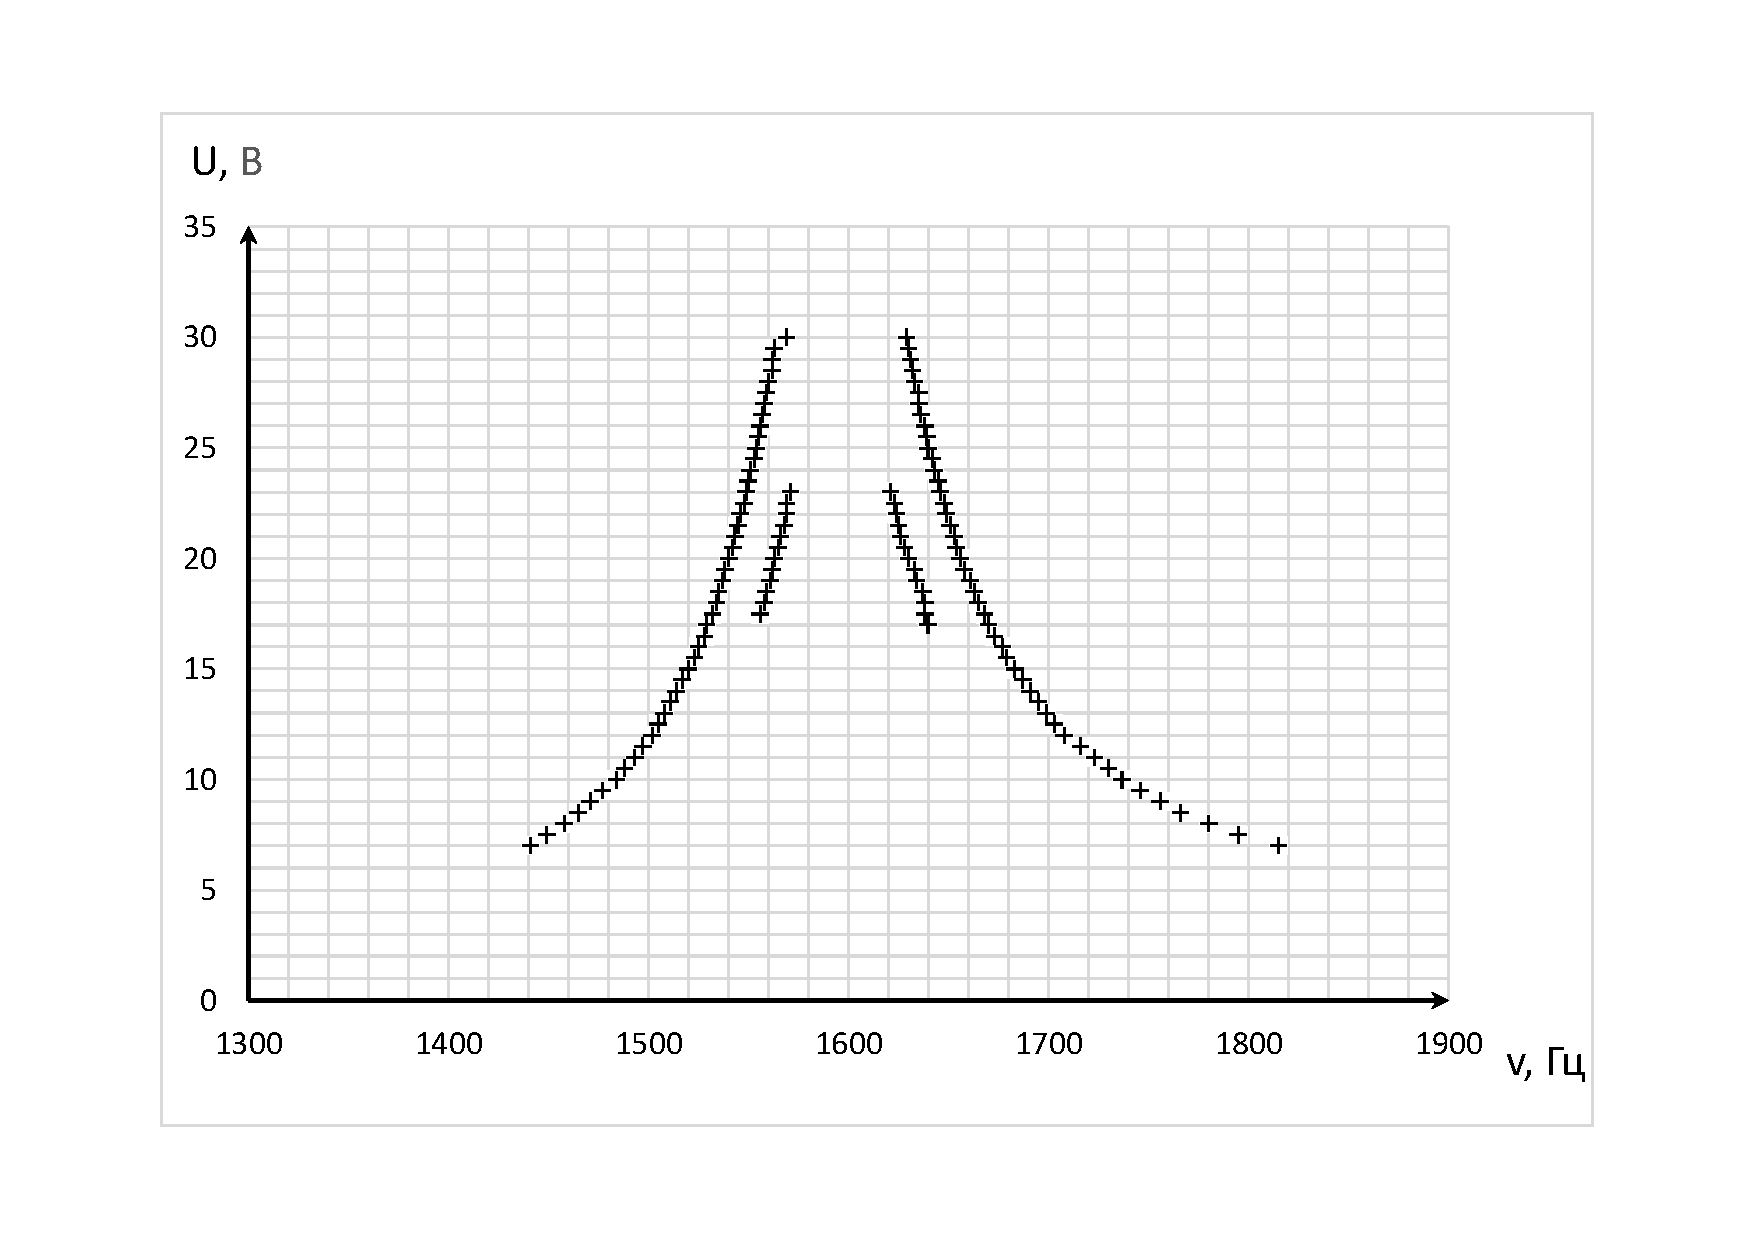
\includegraphics[width = 1.1\textwidth]{graph_of_depence_amplitude_R=0}
			\caption{Резонансная кривая, $R = 0\,$Ом}
			\label{fig:graph_of_depence_amplitude_R=0}
		\end{minipage}
		\hfill
		\begin{minipage}{0.49\textwidth}
			\hspace{-0.5cm}
			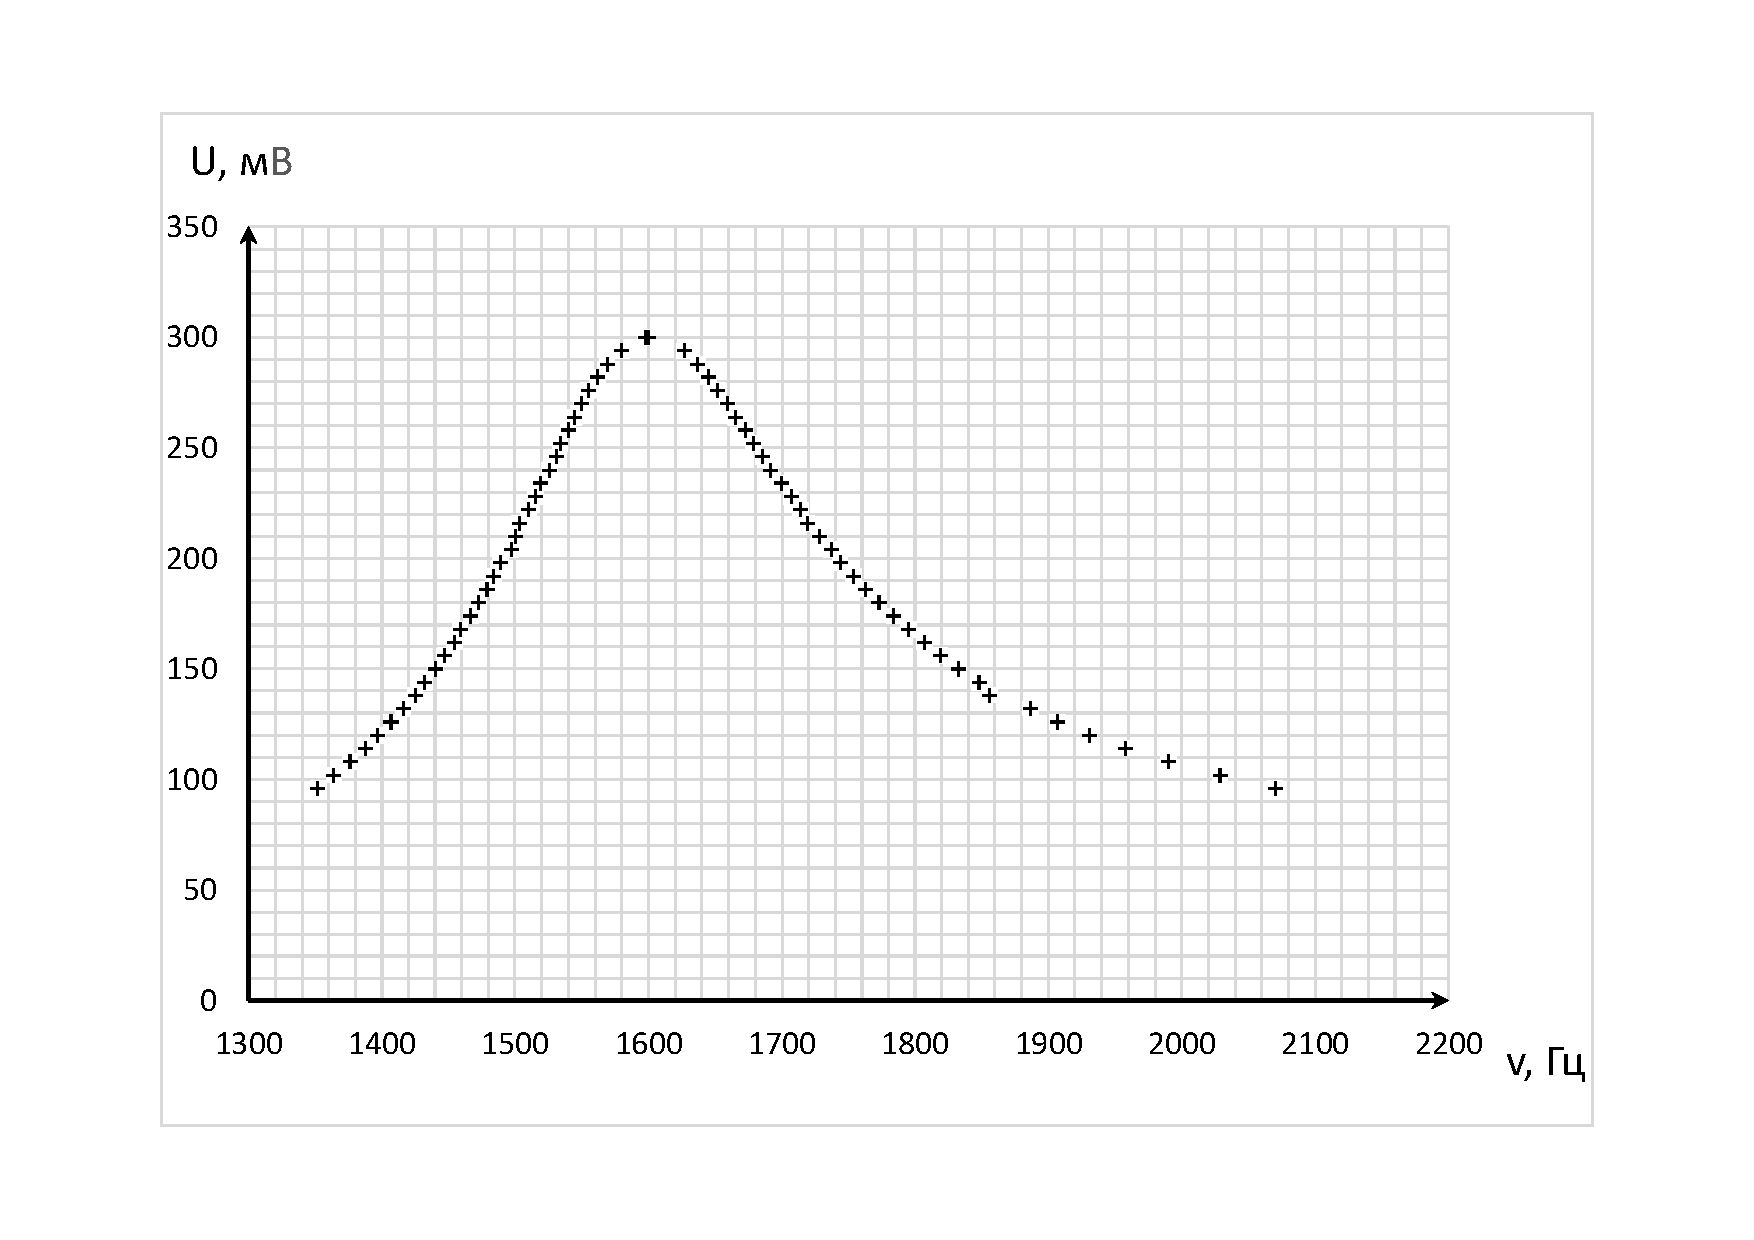
\includegraphics[width = 1.1\textwidth]{graph_of_depence_amplitude_R=100}
			\caption{Резонансная кривая, $R = 100\,$Ом}
			\label{fig:graph_of_depence_amplitude_R=100}
		\end{minipage}
	\end{figure}
	
	Как видно из (рис \ref{fig:graph_of_depence_amplitude_R=0}), измерения были проведены некорректно. Повторная серия измерений зависимости амплитуды напряжения от частоты (точки, лежащие "внутри" кривой) показывает, что изначально выбранная резонансная частота не совпадала с собственной частотой контура. Вернее, корректнее было бы сказать, что измерения кривой проводились не с максимальной амплитуды, что не позволяет провести измерения добротности, так как довольно проблематично определить пик кривой. Для этого будем использовать кривую (часть кривой), полученную при повторном измерении и изображенную на (рис. )
	
	\begin{figure}[h!]
		\centering
		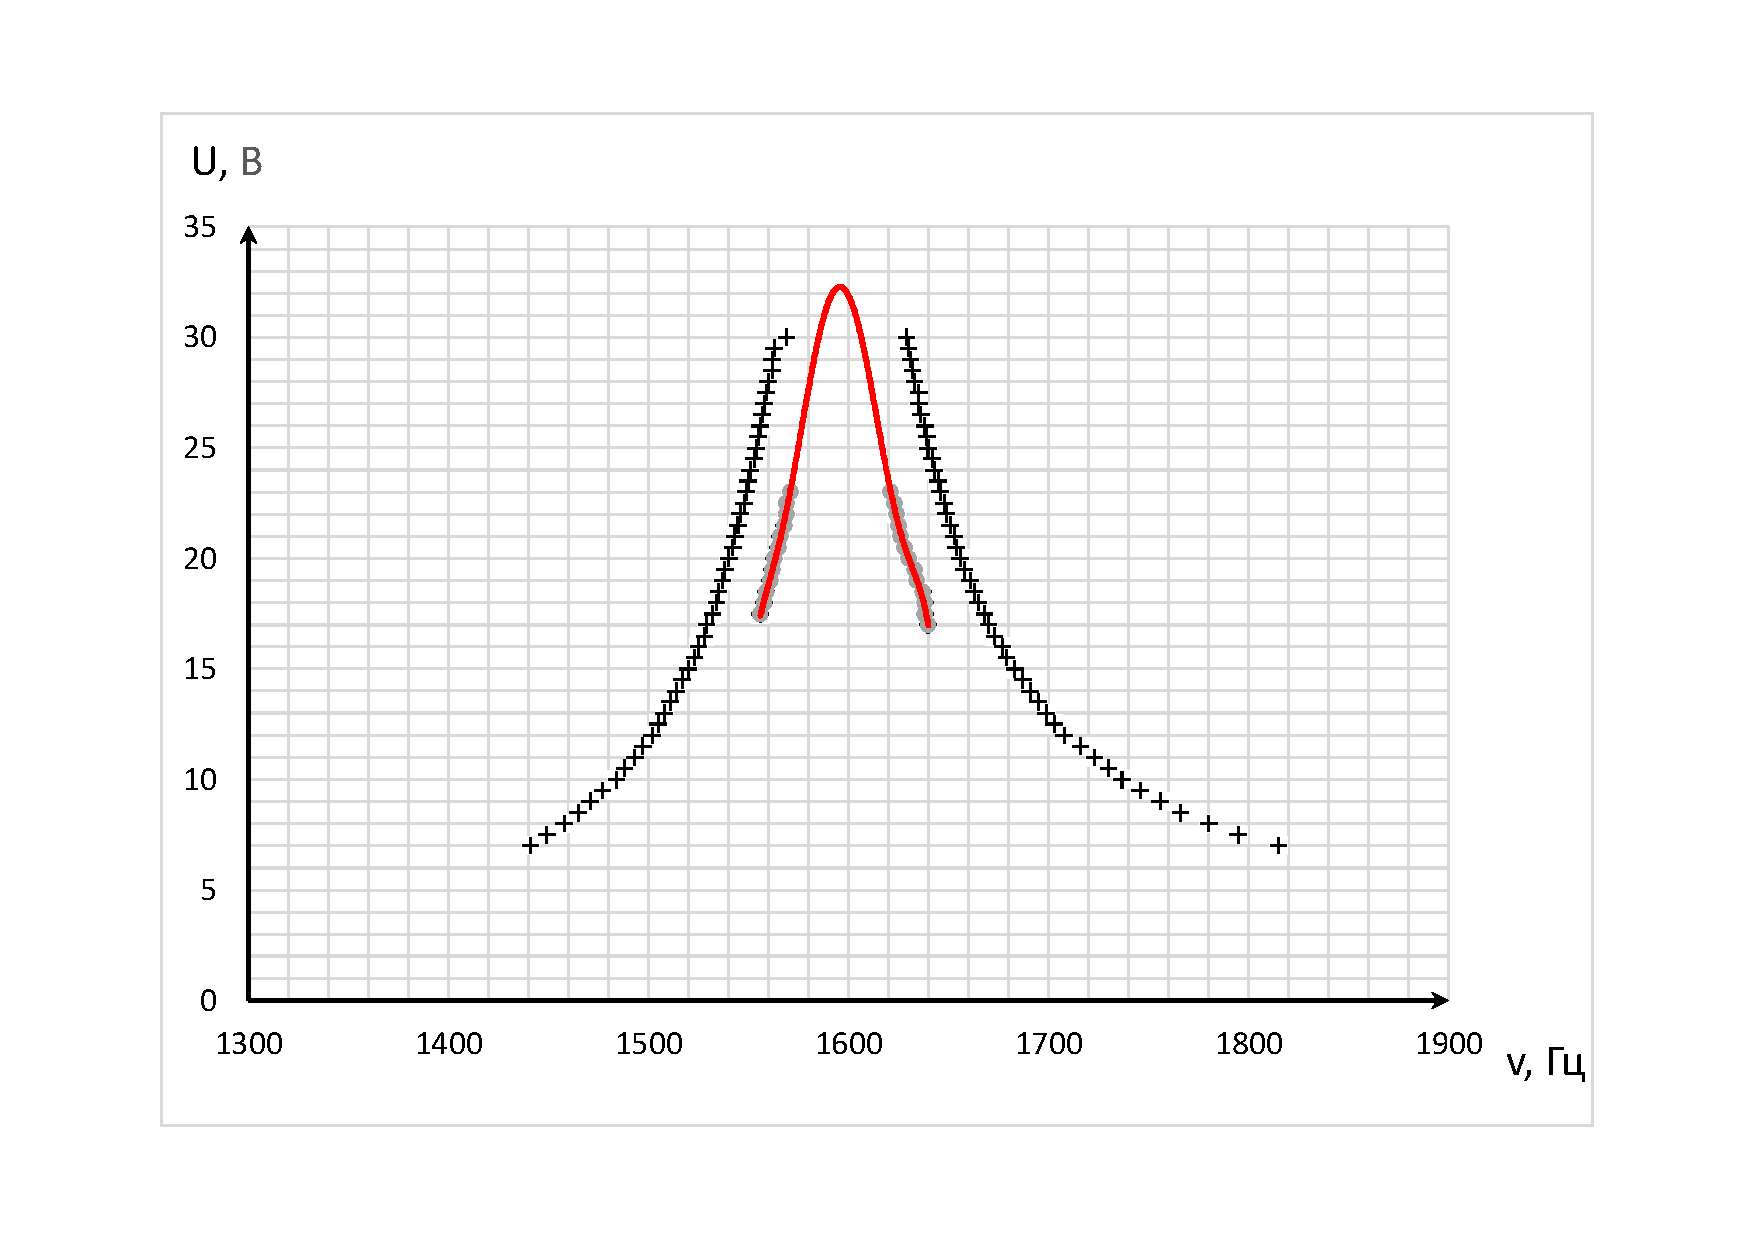
\includegraphics[width = 0.75\textwidth]{graph_of_depence_amplitude_R=0_modiff}
		\caption{экстраполированная резонансная кривая для $R = 0\,$ Ом}
		\label{fig:graph_of_depence_amplitude_R=0_modiff}
	\end{figure}	
	
	Обоснованность использования данной экстраполированной кривой заключается в том, что для определения добротности нам необходимо знать зависимость амплитуды напряжения от частоты только в интервале амплитуд $U \sim \frac{\sqrt{2}}{2}U_{0}$, а так как данная вторая серия измерений и была приведена для данного диапазона амплитуд, то ее использование вполне оправдано.
	
	\subsection{Исследование процессов установления и затухания колебаний}
	
	Для определения добротности с помощью исследования процессов установления и затухания вынужденных колебаний необходимо получить зависимость амплитуды вынужденных колебаний в режиме генератора "цуги".
	
	Для получения зависимости используем осциллограф. С его помощью получаем следующие зависимости (рис. \ref{fig:measuring_Q_on_grown} и \ref{fig:measuring_Q_on_decrease}).
	
	\newpage
	
	\begin{figure}[t!]
		\begin{minipage}{0.49\textwidth}
			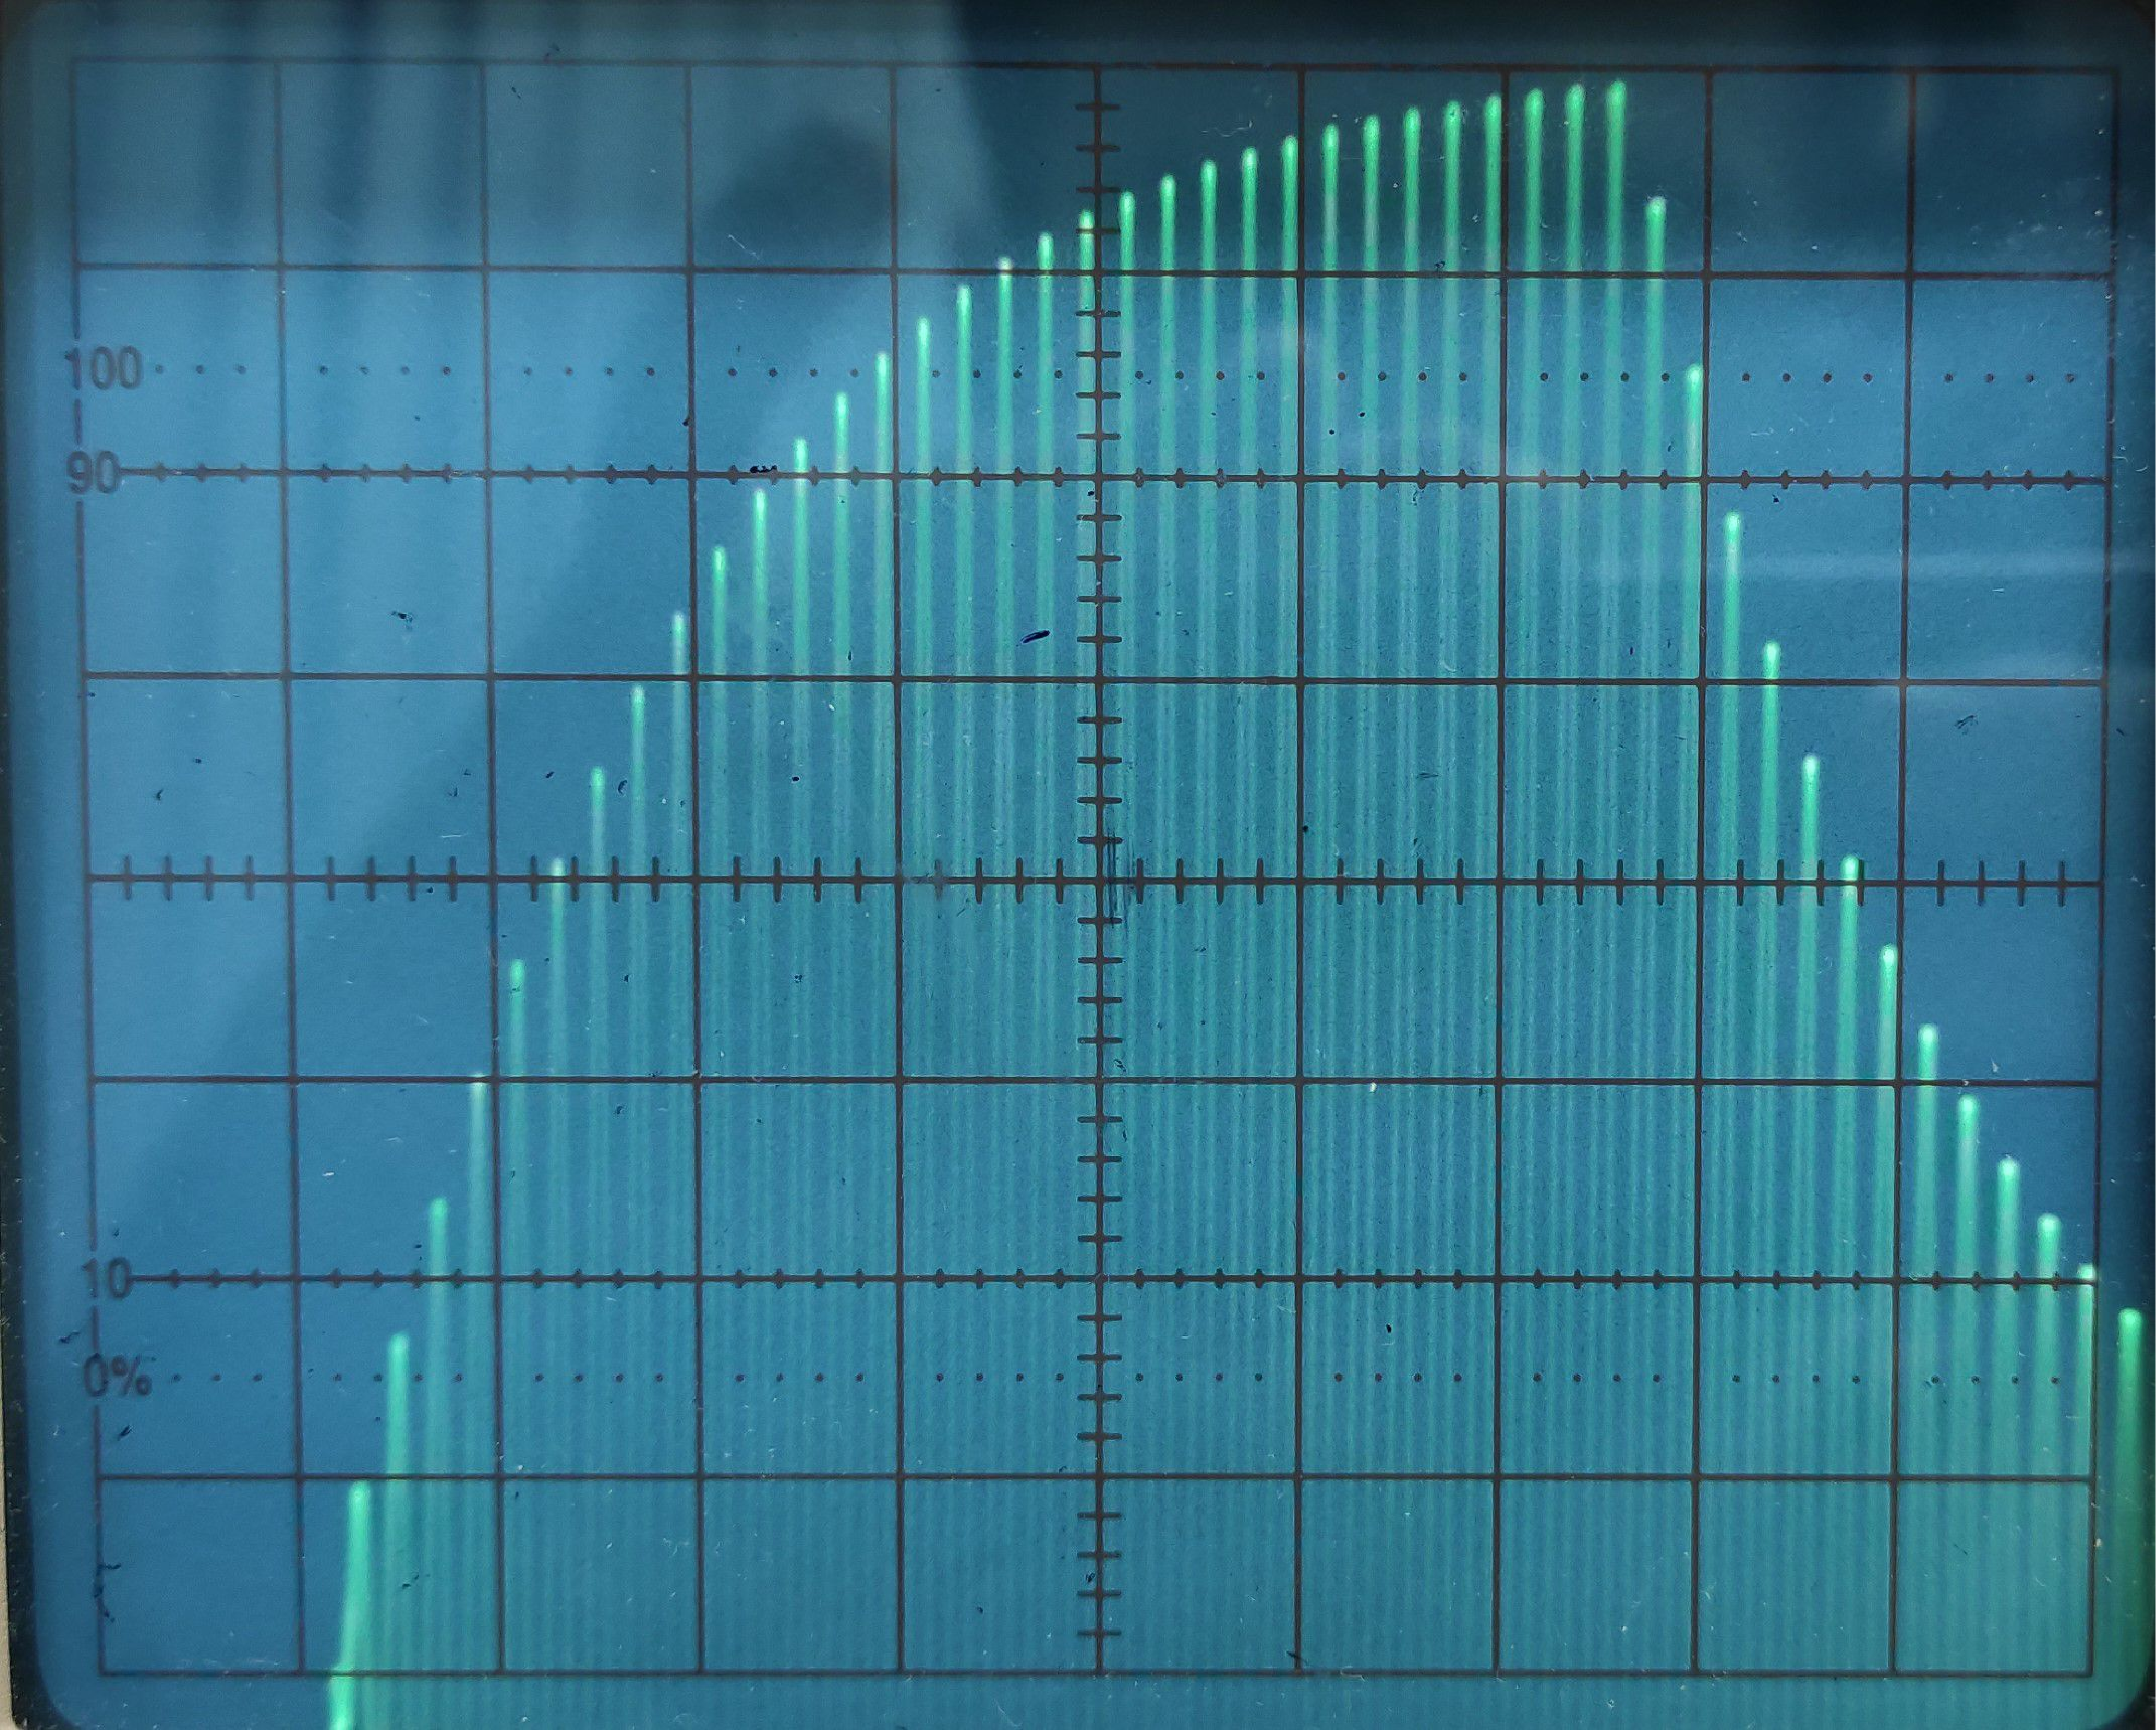
\includegraphics[width = 1.0\textwidth]{measuring_Q_on_grown}
			\caption{зависимость амплитуды напряжения от времени при установлении колебаний}
			\label{fig:measuring_Q_on_grown}
		\end{minipage}
		\hfill
		\begin{minipage}{0.49\textwidth}
			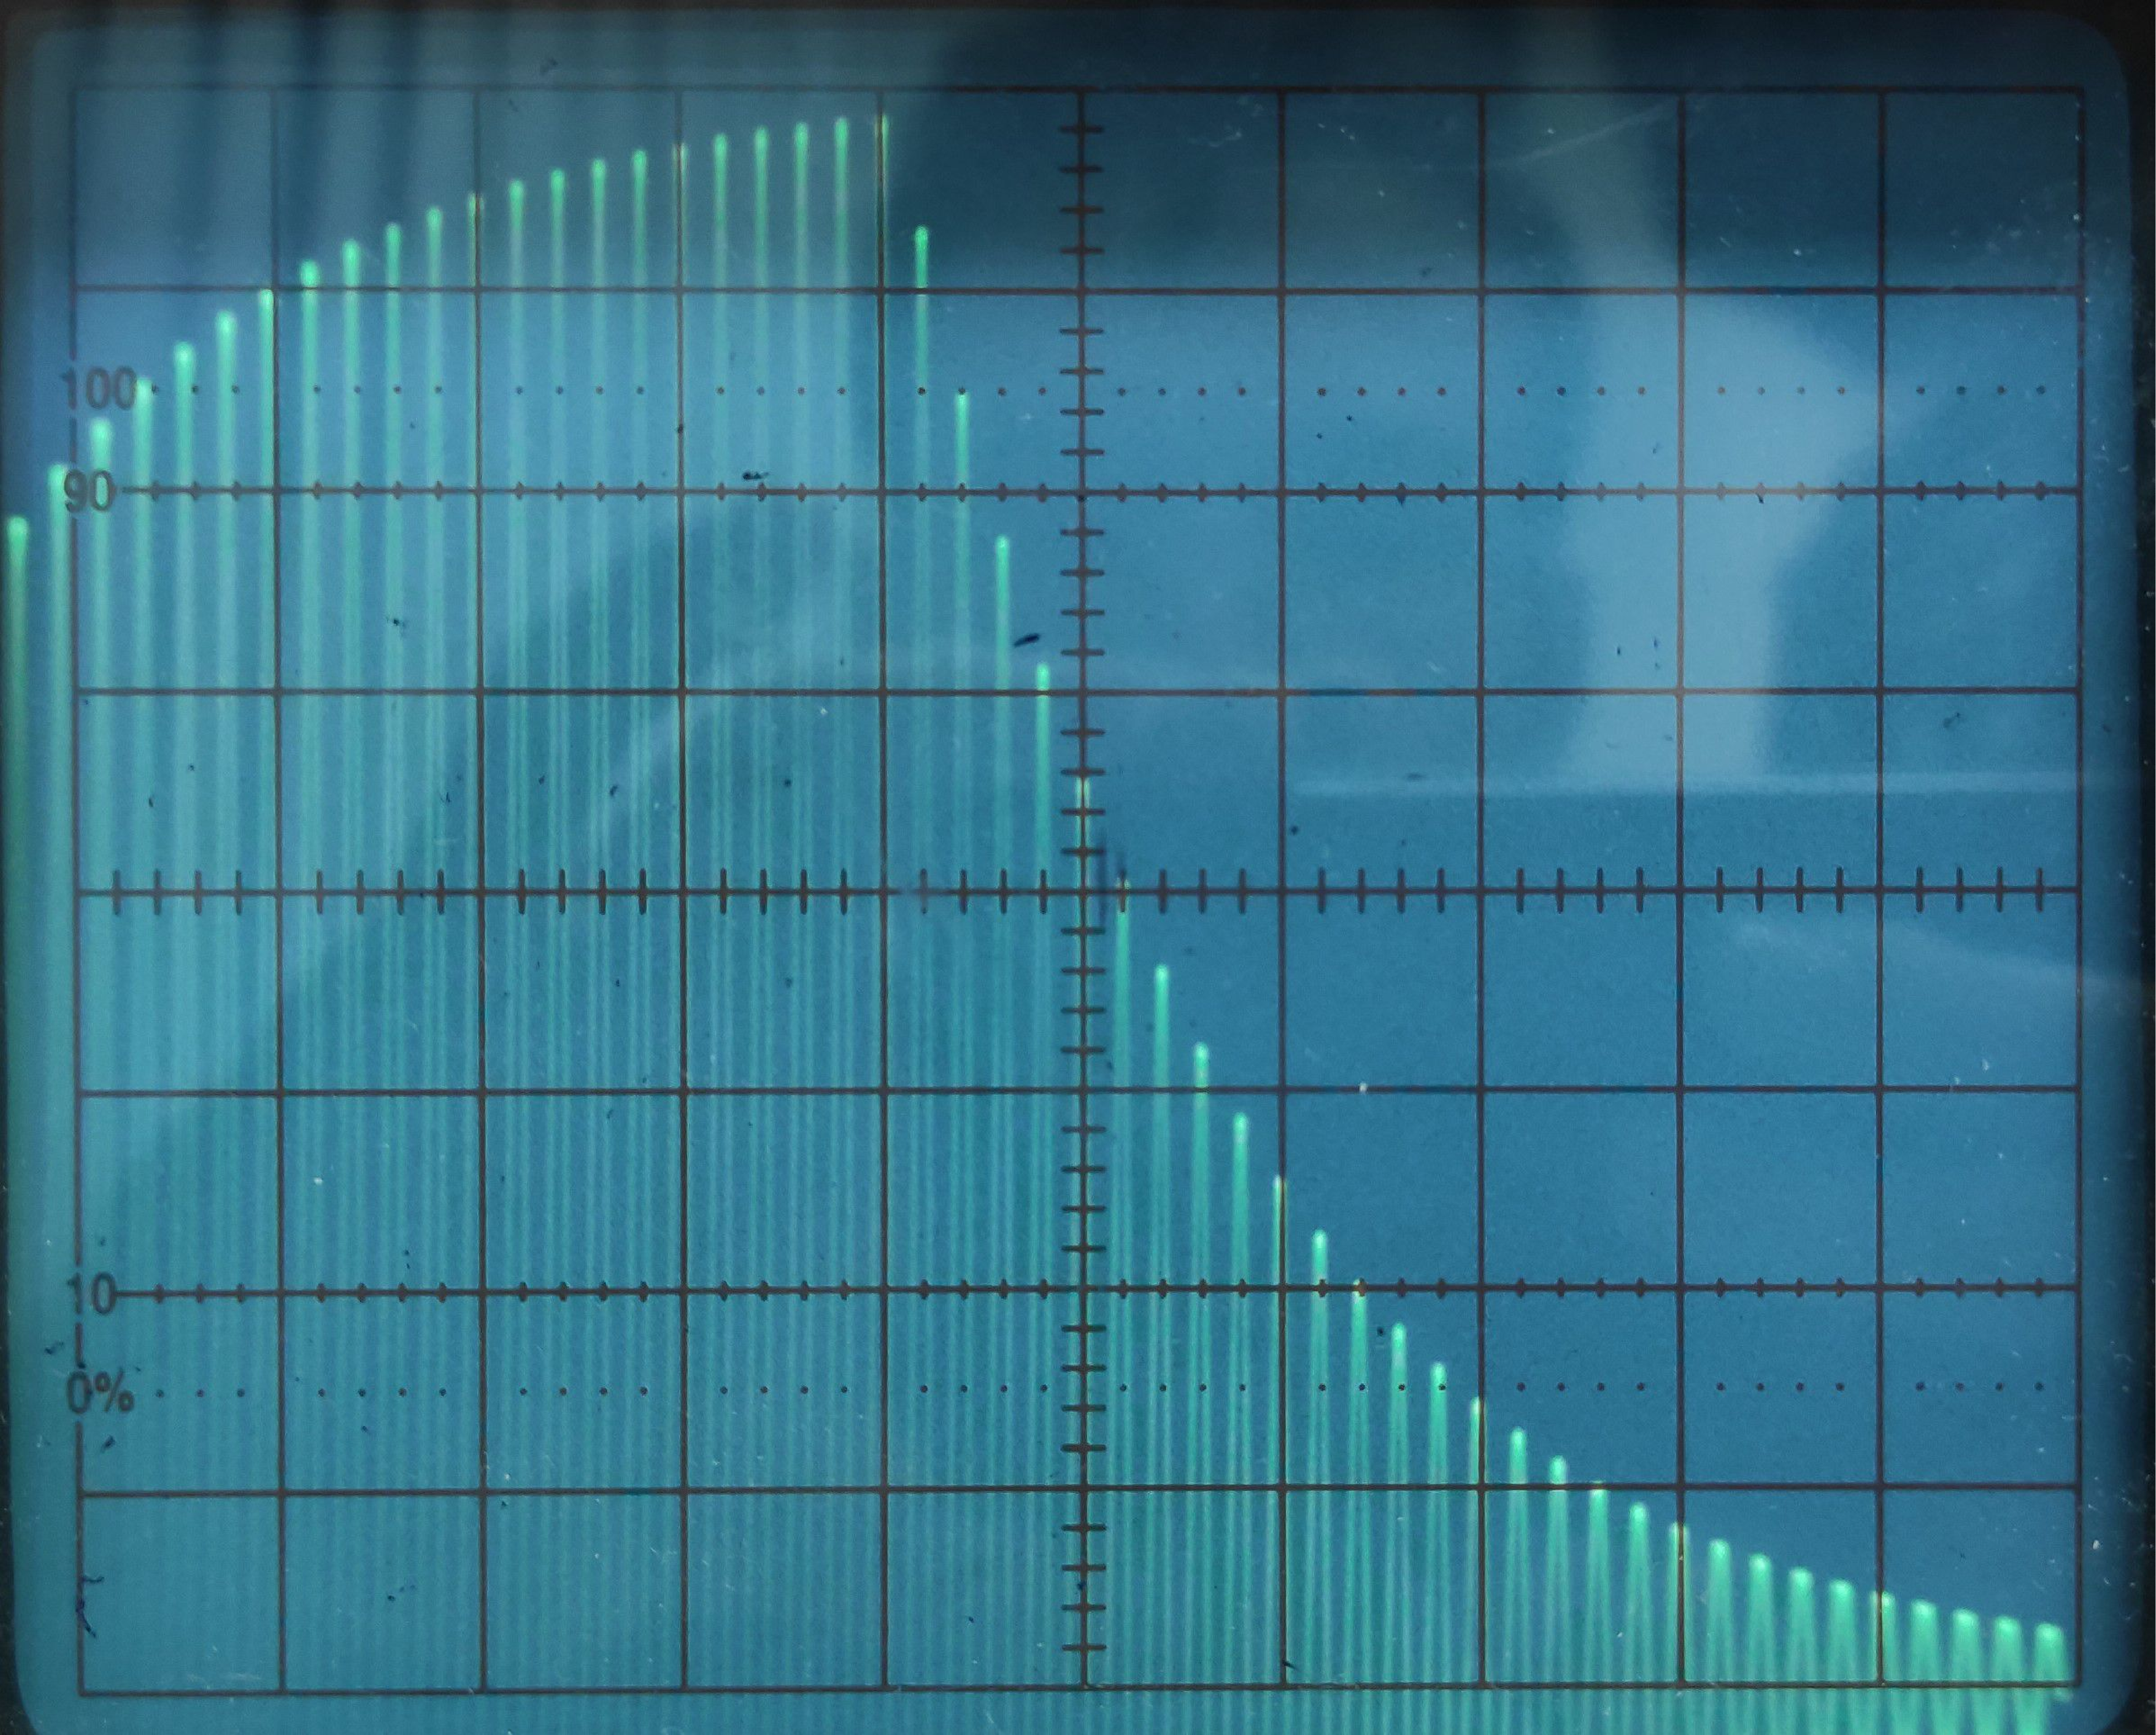
\includegraphics[width = 1.0\textwidth]{measuring_Q_on_decrease}
			\caption{зависимость амплитуды напряжения от времени при затухании колебаний}
			\label{fig:measuring_Q_on_decrease}
		\end{minipage}
	\end{figure}
	
	На основе полученных изображений получим зависимость амплитуд напряжений в процессе установления колебаний (Таблица \ref{tab:Q_measuring_on_grown}) и затухания колебаний (Таблица \ref{tab:Q_measuring_on_decrease})
	
	\begin{table}[h!]
\centering
\begin{tabular}{|l|l|l|l|l|l|l|l|l|l|l|l|l|l|l|l|l|l|l|l|l|}
\hline
n          & 1 & 2 & 3  & 4  & 5  & 6  & 7  & 8  & 9  & 10 & 11 & 12 & 13 & 14 & 15 & 16 & 17 & 18 & 19 & 20 \\ \hline
$U_{n}$, дел & 5 & 8 & 12 & 15 & 17 & 20 & 23 & 25 & 26 & 28 & 29 & 31 & 32 & 33 & 34 & 35 & 35 & 36 & 37 & 37 \\ \hline
\end{tabular}
\caption{Результаты измерения зависимости амплитуды вынужденных колебаний при их установлении}
\label{tab:Q_measuring_on_grown}
\end{table}	




\begin{table}[h!]
\centering
\begin{tabular}{|l|l|l|l|l|l|l|l|l|l|l|l|l|l|l|l|l|l|l|l|l|}
\hline
n          & 1  & 2  & 3  & 4  & 5  & 6  & 7  & 8  & 9  & 10 & 11 & 12 & 13 & 14 & 15 & 16 & 17 & 18 & 19 & 20 \\ \hline
$U_{n}$, дел & 36 & 31 & 28 & 26 & 23 & 20 & 18 & 16 & 14 & 13 & 11 & 10 & 10 & 9  & 8  & 7  & 6  & 6  & 5  & 4  \\ \hline
\end{tabular}
\caption{Результаты измерения зависимости амплитуды вынужденных колебаний при их установлении}
\label{tab:Q_measuring_on_decrease}
\end{table}

	\section{Получение добротности контура и определение погрешностей}
	
	\subsection{Метод резонансных кривых}
		
		Для получения добротности методом исследования резонансных кривых получим с использованием формулы (\ref{eq:equation_1}) значения добротности вблизи искомого диапазона амплитуд, после чего вычислить погрешности косвенного измерения. Для этого построим графики зависимостей $\frac{U_{R=0}}{U_{R=0, 0}} = f\left(\frac{\nu}{\nu_{0}}\right)\ \ \text{и} \ \ \frac{U_{R=100}}{U_{R=100, 0}} = f\left(\frac{\nu}{\nu_{0}}\right)$
		
	\begin{figure}[h!]
		\centering
		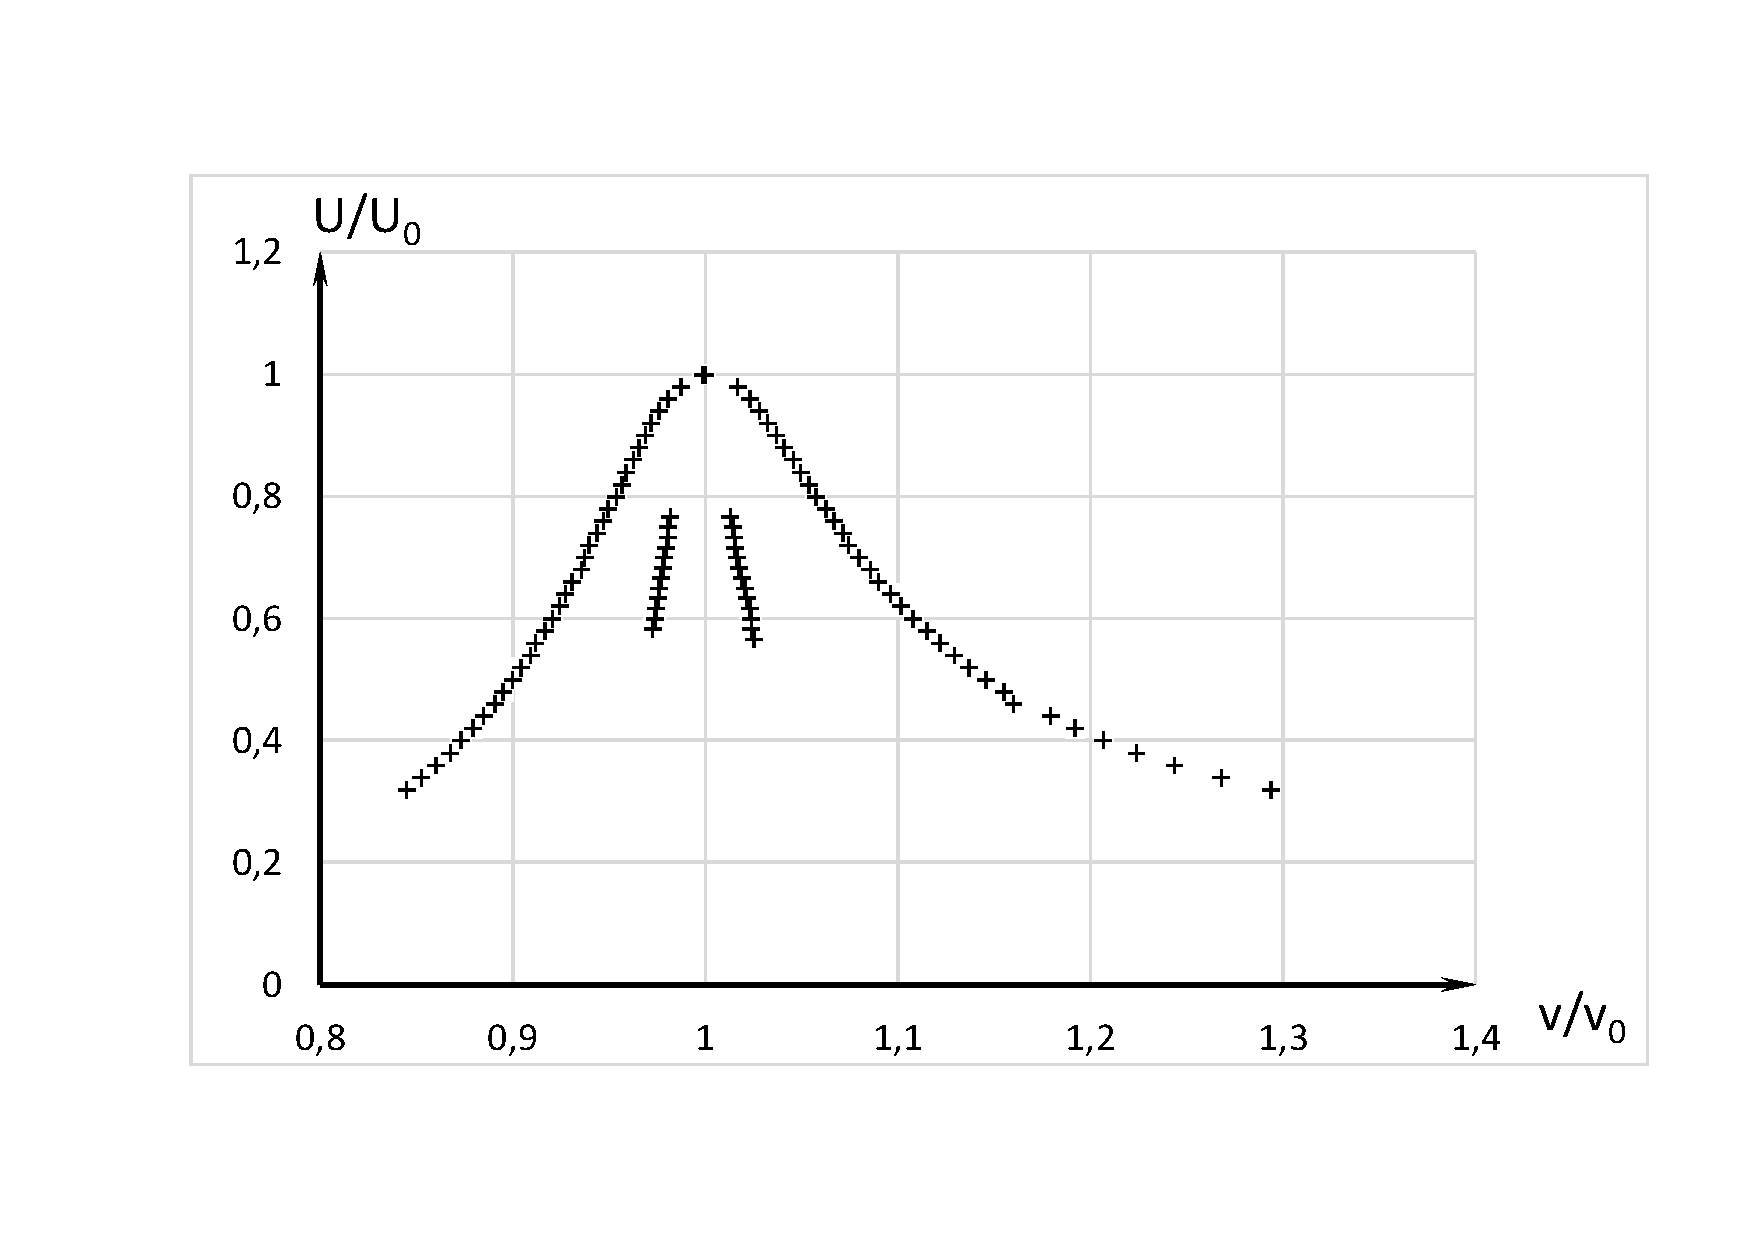
\includegraphics[width = 0.5\textwidth]{graph_of_depence_relative}
		\caption{График зависимости $\frac{U}{U_{0}} = f\left(\frac{\nu}{\nu_{0}}\right)$ для двух конфигураций контура: $R = 0$ Ом и $R = 100$ Ом}
		\label{fig:graph_of_depence_relative}
	\end{figure}
	
	Результаты вычисления добротности с использованием формулы (\ref{eq:equation_1}) занесем в таблицу (\ref{tab:Q_from_resonance_curve}) для соответствующих значений $R$
	
	\begin{table}[h!]
\centering
\begin{tabular}{|l|l|l|}
\hline
$R,$ Ом & $Q$ & $\sigma_{Q}$ \\ \hline
0       & 50,1           & 10,4                      \\ \hline
100     & 14,7           & 3,7                       \\ \hline
\end{tabular}
\caption{Результаты определения добротности методом исследования резонансных кривых}
\label{tab:Q_from_resonance_curve}
\end{table}

	\subsection{Метод исследования процессов установления и затухания колебаний}
	
	\begin{table}[h!]
\centering
\begin{tabular}{|l|l|l|l|l|l|l|l|l|l|l|l|l|l|l|l|}
\hline
$\Theta_{1}$ & 0,090 & 0,112 & 0,112 & 0,105 & 0,112 & 0,120 & 0,121 & 0,115 & 0,119 & 0,116 & 0,123 & 0,123 & 0,124 & 0,126 \\ \hline
$\Theta_{2}$ & 0,150 & 0,126 & 0,108 & 0,112 & 0,118 & 0,116 & 0,116 & 0,118 & 0,113 & 0,119 & 0,116 & 0,107 & 0,107 & 0,107 \\ \hline
\end{tabular}
\caption{Результаты измерения логарифмического декремента затухания для $R = 0$ Ом}
\label{tab:theta_measuring}
\end{table}

	Определив среднее значение величин $\Theta_{1}$ и $\Theta_{2}$, а также воспользовавшись соотношениями:
	
	\begin{equation}
		f = \ln\left(\frac{U_{1}}{U_{2}}\right), \Rightarrow \sigma_{f} = \sqrt{\left(\frac{\partial f}{\partial U_{1}} \sigma_{U}\right)^2 + \left(\frac{\partial f}{\partial U_{2}} \sigma_{U}\right)^{2}} = \frac{\sigma_{U}\sqrt{U_{1}^{2} + U_{2}^{2}}}{U_{1}U_{2}}
	\end{equation}
	
	\begin{equation}
		f = \ln\left(\frac{U_{0} - U_{1}}{U_{0} - U_{2}}\right), \Rightarrow \sigma_{f} = \sqrt{\left(\frac{\partial f}{\partial U_{1}} \sigma_{U}\right)^2 + \left(\frac{\partial f}{\partial U_{2}} \sigma_{U}\right)^{2}} = \frac{\sigma_{U}\sqrt{\left(U_{0} - U_{1}\right)^{2} + \left(U_{0} - U_{2}\right)^{2}}}{\left(U_{0} - U_{1}\right)\left(U_{0} - U_{2}\right)}
	\end{equation}
	
	Получаем:
	
	\begin{table}[h!]
\centering
\begin{tabular}{|l|l|l|l|}
\hline
$Q_{1}$ & $Q_{2}$ & $\sigma_{Q_{1}}$ & $\sigma_{Q_{2}}$ \\ \hline
52,8    & 54,7    & 5,2              & 5,9              \\ \hline
\end{tabular}
\caption{Результаты определения добротности контура при $R = 0$ Ом}
\label{tab:Q_measuring_on_grown_and_decrease_results}
\end{table}

Так как исследование процессов установления и затухания колебаний проводились только для конфигурации контура с $R = 0$ Ом, то определить таким методом добротность при $R = 100$ Ом не представляется возможным ввиду отсутствия данных.

	\subsection{Теоретическое определение добротности контура}
	
	Для теоретического определения добротности контура используем следующее соотношение:
	
	\begin{equation}
		Q = \frac{\sqrt{L}}{R\sqrt{C}}
	\end{equation}
	
	А также соотношение:
	
	\begin{equation}
		\sigma_{Q} = \sqrt{\left(\frac{\partial Q}{\partial R} \sigma_{R}\right)^{2}+ \left(\frac{\partial Q}{\partial L} \sigma_{L}\right)^{2} + \left(\frac{\partial Q}{\partial C} \sigma_{C}\right)^{2}}
	\end{equation}
	
	\begin{equation}
		\sigma_{Q} = \sqrt{\frac{\sigma_{R}^{2}L}{2R^{4}C} + \frac{\sigma_{L}^{2}}{2R^{2}LC}+ \frac{\sigma_{C}^{2}L}{2R^{2}C^{3}}} 
	\end{equation}
	
	Получаем итоговую таблицу:
	
	\begin{table}[h!]
\centering
\begin{tabular}{|l|l|l|l|l|}
\hline
$R,$ Ом & $Q_{\text{резон. кривая}}$ & $Q_{\text{установление кол.}}$ & $Q_{\text{затухание кол.}}$ & $Q_{\text{теор}}$             \\ \hline
0       & $50,1 \pm 10,4$            & $52,8 \pm 5,2$                 & $54,7 \pm 5,9$              & $50,3 \pm 1,1$ \\ \hline
100     & $14,7 \pm 3,7$             & --                             & --                          & $10,0 \pm 0,7$                \\ \hline
\end{tabular}
\caption{Итоговая таблица с результатами измерения добротности}
\label{tab:final_table}
\end{table}

	\section{Исследование картины биений вблизи собственной частоты контура}
	
	Для получения картины биений вблизи собственной частоты контура установим на генераторе частоту такую, что графиком сигнала на осциллографе будет синусоида с максимальной амплитудой. Затем, немного отклонив частоту генератора на экране осциллографа получим картину биений, представленную на рисунке 
	
	\begin{figure}[h!]
		\centering
		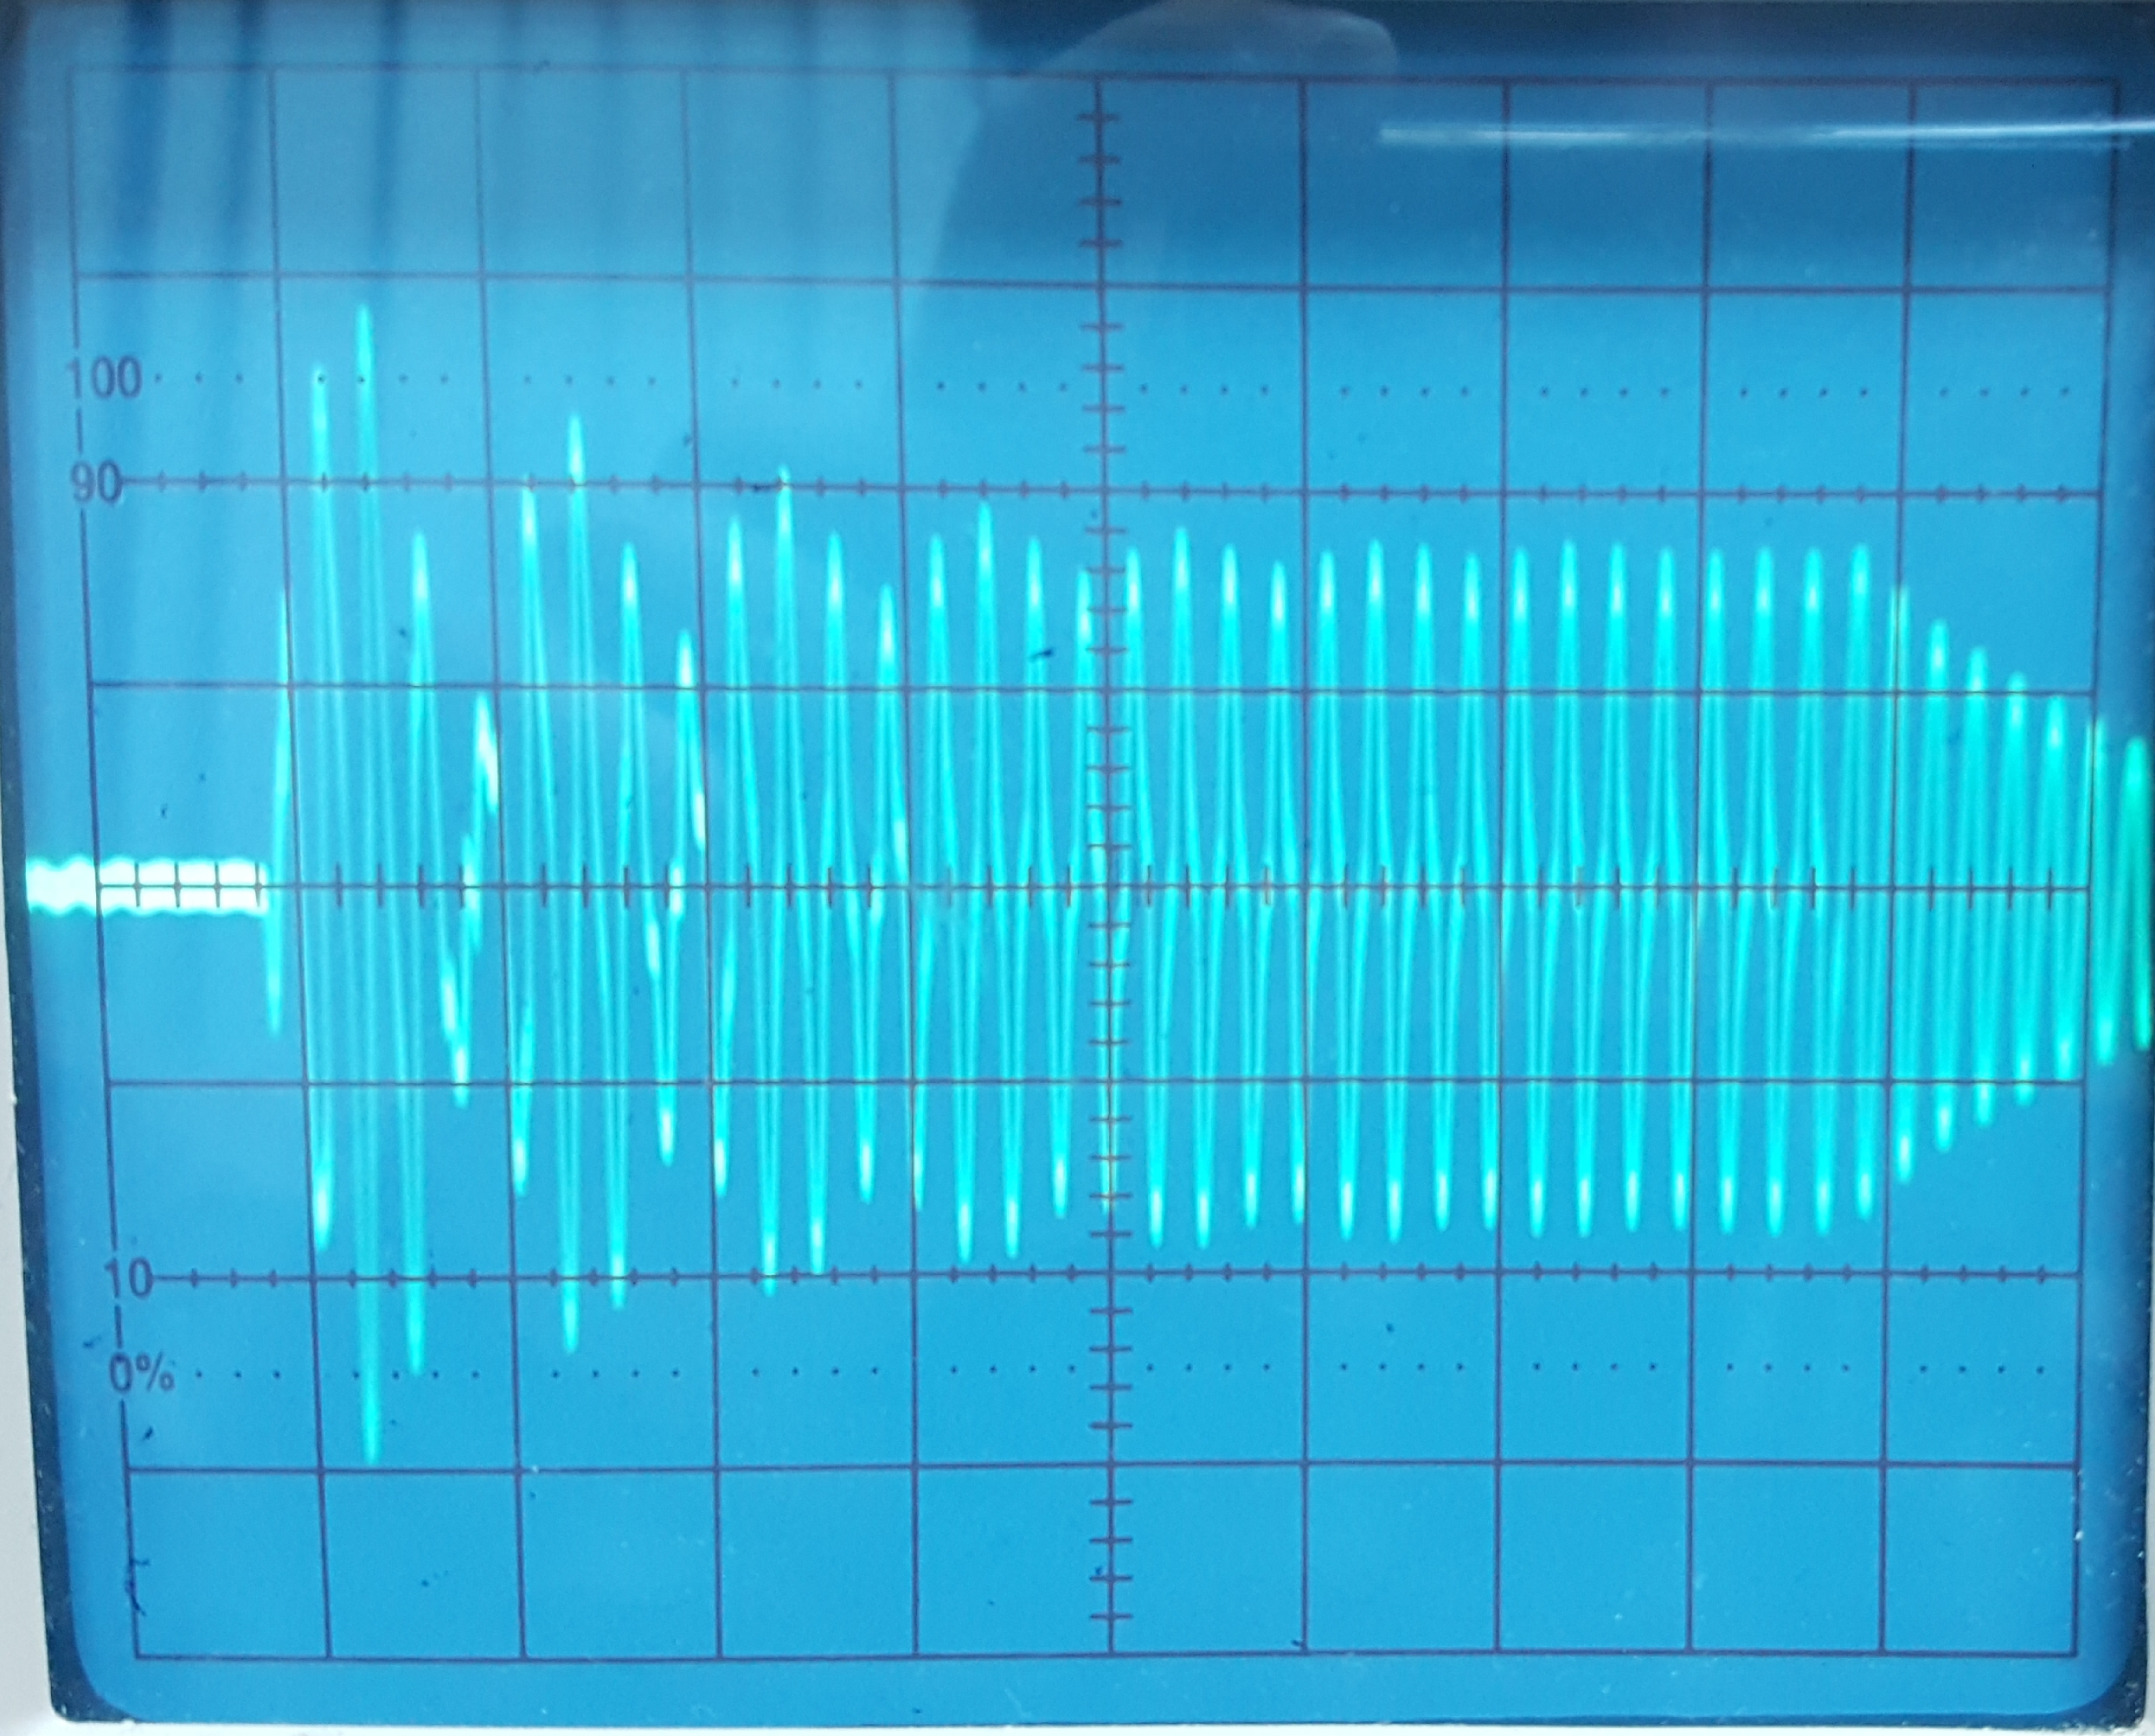
\includegraphics[width = 0.95\textwidth]{beats}
		\caption{Картина биений вблизи собственной частоты контура}
		\label{fig:beats}	
	\end{figure}
	
	\newpage
	
	\section{Итоги}
	
	\begin{enumerate}
		\item В данной работе проведены измерения добротности колебательной системы, представляющей собой электрический колебательный контур, состоящий из последовательно соединенных катушки, резистора переменной емкости (магазин сопротивлений) и конденсатора. Получены значения добротности контура в различных конфигурациях: при $R = 0$ Ом и $R = 100$ Ом.
		\item Проведены измерения погрешностей определения добротности колебательной системы. Установлено, что значения, полученные всеми способами определения добротности колебательной системы, предложенными для проверки, согласуются с теоретическими значениями добротности в различных конфигурациях.
		\item Наибольшая погрешность возникла при определении добротности с помощью метода анализа резонансной кривой, так как для хорошей статистической обеспеченности полученного результата пришлось брать довольно широкий диапазон частот, для которых проводилось измерение, что привело к увеличению погрешности. кроме того, отдельно отметим тот факт, что при измерении резонансной кривой для конфигурации с нулевым сопротивлением была совершена неточность, которая привела к искусственному расширению кривой (подробно данная ошибка описана в п. 3.1)
		\item Относительная точность всех измерений не превосходит $\varepsilon_{max} \approx 20 \%$
		\item Наибольший вклад в определение погрешности полученных величин внесли статистические (случайные) ошибки, а так же ошибки, связанные с определением величин амплитуд сигнала на экране осциллографа.
		\item Установлено, что при $R = 0$ Ом предпочтительнее проводить измерения добротности методом исследования процессов установления и затухания колебаний, нежели исследованием резонансной кривой. 
		
		Для $R = 100$ Ом недостаточно данных для установления приоритета.
		\item Полученная картина биений соответствует теоретически предсказанной картине.
	\end{enumerate}


	
\end{document}
